\documentclass[11pt]{article}

\usepackage[margin=1in]{geometry}
\usepackage{amsmath,amssymb,booktabs}
\usepackage{graphicx}
\usepackage{hyperref}
\usepackage{enumitem}
\usepackage{xcolor}

\hypersetup{
  colorlinks=true,
  linkcolor=blue,
  urlcolor=blue,
  citecolor=blue
}

\title{Online Ride Dispatch Optimizer\\Technical Report}
\author{Lola Rapoport}
\date{\today}

\begin{document}

\maketitle

\begin{abstract}
This report describes a simulator for real-time ride dispatch on a graph. Riders arrive online, drivers move through a road-network abstraction, and dispatch policies must assign available drivers to pending riders while balancing pickup cost, rider waiting time, rejection rate, and fleet utilization. The project implements five policies: greedy nearest-driver matching, fixed-interval batch matching, min-cost bipartite matching, an online primal-dual style heuristic, and a learned demand-aware heuristic. The simulator is intended as a practical demonstration of online algorithms, matching, stochastic demand modeling, and operational tradeoffs relevant to algorithmic mobility platforms.
\end{abstract}

\section{Motivation}

Ride dispatch is an online decision problem: requests arrive without full knowledge of the future, and each assignment consumes a scarce resource, namely driver availability in space and time. A locally cheap assignment can create future scarcity in a high-demand zone, while excessive batching can improve optimization quality at the cost of rider delay. This makes the domain a good applied setting for online algorithms, primal-dual thinking, min-cost assignment, and empirical evaluation.

\section{System Model}

The city is represented as an undirected graph
\[
G = (V, E),
\]
where each node is a location and each edge has unit travel time. The implementation uses a grid graph by default, but the simulator is written against NetworkX graphs and can support richer road-network inputs.

At each discrete time step \(t = 0, 1, \ldots, H-1\), a random number of riders arrives. A rider
\[
r = (o_r, d_r, a_r, w_r^{\max})
\]
has origin \(o_r \in V\), destination \(d_r \in V\), arrival time \(a_r\), and maximum allowed wait \(w_r^{\max}\). A driver
\[
i = (x_i(t), b_i(t))
\]
has current node \(x_i(t)\) and busy-until time \(b_i(t)\). Driver \(i\) is available at time \(t\) when \(b_i(t) \leq t\).

The shortest-path distance between two graph nodes is denoted by
\[
\operatorname{dist}(u,v).
\]
If driver \(i\) is assigned to rider \(r\) at time \(t\), the pickup time is
\[
p_{ir}(t) = \operatorname{dist}(x_i(t), o_r),
\]
the trip time is
\[
\tau_r = \operatorname{dist}(o_r, d_r),
\]
and the rider's total wait is modeled as
\[
W_r(t) = (t - a_r) + p_{ir}(t).
\]
The driver becomes unavailable until \(t + p_{ir}(t) + \tau_r\), then reappears at \(d_r\).

\section{Objective}

The simulator evaluates policies empirically instead of solving a single offline objective. The central tradeoff is captured by the following stylized cost:
\[
\min \sum_{r \in M} \left(\alpha W_r + \beta p_{ir}\right)
  + \lambda \sum_{r \in R} \mathbf{1}\{r \text{ rejected}\}
  - \gamma \cdot \operatorname{Utilization},
\]
where \(M\) is the set of matched riders and \(R\) is the set of all arrived riders. In practice, the report focuses on interpretable metrics:

\begin{itemize}[nosep]
  \item mean rider wait time,
  \item 95th percentile rider wait time,
  \item mean pickup distance,
  \item rejection rate,
  \item completion rate,
  \item fleet utilization.
\end{itemize}

\section{Arrival Process}

Rider arrivals are generated by a non-homogeneous Poisson process. The expected arrivals at time \(t\) are
\[
\lambda(t) = \lambda_0 \left(1 + m \cdot q(t)\right),
\]
where \(\lambda_0\) is the base arrival rate, \(m\) is a peak multiplier, and \(q(t)\) is a periodic demand curve. Spatial demand is biased toward configurable hot spots. This creates more realistic imbalances than uniform arrivals and allows the demand-aware policy to have a meaningful signal.

\section{Algorithms}

\subsection{Greedy Nearest-Driver Matching}

The greedy policy processes pending riders in arrival order and assigns each rider the closest currently available driver:
\[
i^*(r) = \arg\min_{i \in A(t)} \operatorname{dist}(x_i(t), o_r).
\]
It is fast, online, and easy to reason about, but it does not account for the joint structure of multiple simultaneous riders. It can make locally optimal choices that are globally suboptimal.

\subsection{Batch Matching Every T Seconds}

The batch policy only matches at times divisible by a fixed interval \(T\). At batch time, it solves a min-cost assignment over the currently available drivers and pending riders. Batching can improve matching quality when several riders are present simultaneously, but it intentionally delays riders between batch boundaries.

\subsection{Min-Cost Bipartite Matching}

At every time step, the min-cost policy builds a bipartite graph between available drivers and pending riders. The assignment cost is
\[
c_{ir}(t) = \alpha \operatorname{dist}(x_i(t), o_r) - \eta (t - a_r),
\]
where the wait credit \(\eta\) prioritizes riders who have already waited. The implementation solves the linear assignment problem with SciPy's Hungarian algorithm:
\[
\min \sum_{i,r} c_{ir}(t) x_{ir}
\]
subject to each driver and rider being used at most once.

\subsection{Online Primal-Dual Style Heuristic}

The primal-dual inspired policy maintains nonnegative zone-level shadow prices. Each zone \(z\) receives a dual variable \(\pi_z(t)\) that increases when pending rider demand exceeds available driver supply:
\[
\pi_z(t+1) =
\max\{0, \rho \pi_z(t) + s(D_z(t) - S_z(t))\},
\]
where \(D_z(t)\) is pending demand, \(S_z(t)\) is available supply, \(\rho\) is a decay factor, and \(s\) is a step size.

The assignment score adjusts pickup cost using both the driver's current zone and the rider's origin zone:
\[
\operatorname{score}_{ir}(t) =
\operatorname{dist}(x_i(t), o_r)
+ \pi_{z(x_i)}(t)
- 1.25\pi_{z(o_r)}(t)
- \eta(t-a_r).
\]
This heuristic discourages draining drivers from scarce zones and encourages serving high-pressure zones.

\subsection{Learned Demand-Aware Heuristic}

The learned demand-aware policy uses an online exponentially decayed demand forecast. For each zone \(z\),
\[
\hat{d}_z(t+1) = \delta \hat{d}_z(t) + A_z(t),
\]
where \(A_z(t)\) is the number of new arrivals in zone \(z\) and \(\delta\) is a decay rate. The assignment cost reserves drivers in high-demand zones and rewards trips that end near predicted future demand:
\[
c_{ir}(t) =
\operatorname{dist}(x_i(t), o_r)
+ \mu \hat{d}_{z(x_i)}(t)
- \nu \hat{d}_{z(d_r)}(t)
- \eta(t-a_r).
\]
This is intentionally lightweight rather than a full supervised model; it demonstrates the architecture needed to replace the forecast with a trained demand model later.

\section{Complexity}

Let \(m\) be the number of available drivers and \(n\) be the number of pending riders at a time step.

\begin{itemize}[nosep]
  \item Greedy nearest-driver matching computes pairwise distances in \(O(mn)\) time per step.
  \item Min-cost bipartite matching builds an \(m \times n\) cost matrix and solves assignment in \(O(k^3)\), where \(k=\max(m,n)\), after distance lookup.
  \item Batch matching has the same per-batch complexity as min-cost matching but runs only every \(T\) steps.
  \item The primal-dual heuristic updates zone prices in \(O(m+n)\), then sorts candidate pairs, giving \(O(mn\log(mn))\) in the current implementation.
  \item The demand-aware heuristic has the same assignment complexity as min-cost bipartite matching plus lightweight forecast updates.
\end{itemize}

Shortest-path distances are cached by an all-pairs distance oracle for the grid graph, trading memory for fast repeated dispatch queries.

\section{Experimental Setup}

The default experiment uses:

\begin{itemize}[nosep]
  \item a \(16 \times 16\) grid graph,
  \item 45 drivers,
  \item 600 time steps,
  \item base rider arrival rate \(0.28\),
  \item maximum rider wait of 120 seconds,
  \item batch interval \(T=30\) seconds,
  \item fixed random seed for reproducibility.
\end{itemize}

The experiment can be reproduced with:

\begin{verbatim}
python -m ride_dispatch_optimizer.cli \
  --horizon 600 \
  --drivers 45 \
  --grid-width 16 \
  --grid-height 16 \
  --base-rate 0.28 \
  --out outputs/latest
\end{verbatim}

\section{Demonstrated Results}

The repository includes a demonstrated result snapshot under \texttt{docs/}. A fresh experiment writes updated artifacts under \texttt{outputs/latest/}; those can be copied into \texttt{docs/} when the report snapshot should be refreshed.

\begin{table}[h]
\centering
\caption{Policy comparison from the latest generated experiment.}
\label{tab:results}
\IfFileExists{docs/results/summary_table.tex}{\resizebox{\textwidth}{!}{\begin{tabular}{lrrllll}
\toprule
policy & completed & rejected & mean\_wait\_time & p95\_wait\_time & mean\_pickup\_distance & fleet\_utilization \\
\midrule
min-cost-bipartite & 307 & 0 & 2.059 & 6.000 & 2.059 & 0.143 \\
online-primal-dual & 307 & 0 & 2.075 & 6.000 & 2.075 & 0.143 \\
greedy-nearest & 307 & 0 & 2.104 & 6.000 & 2.104 & 0.144 \\
learned-demand-aware & 307 & 0 & 2.121 & 5.000 & 2.121 & 0.144 \\
batch-30s & 298 & 9 & 16.091 & 30.000 & 2.107 & 0.139 \\
\bottomrule
\end{tabular}
}}{
\begin{tabular}{lrrrrrr}
\toprule
Policy & Completed & Rejected & Mean Wait & P95 Wait & Mean Pickup & Utilization\\
\midrule
\multicolumn{7}{c}{Run the experiment command to generate results.}\\
\bottomrule
\end{tabular}
}
\end{table}

\begin{figure}[h]
\centering
\IfFileExists{docs/figures/policy_summary.png}{
  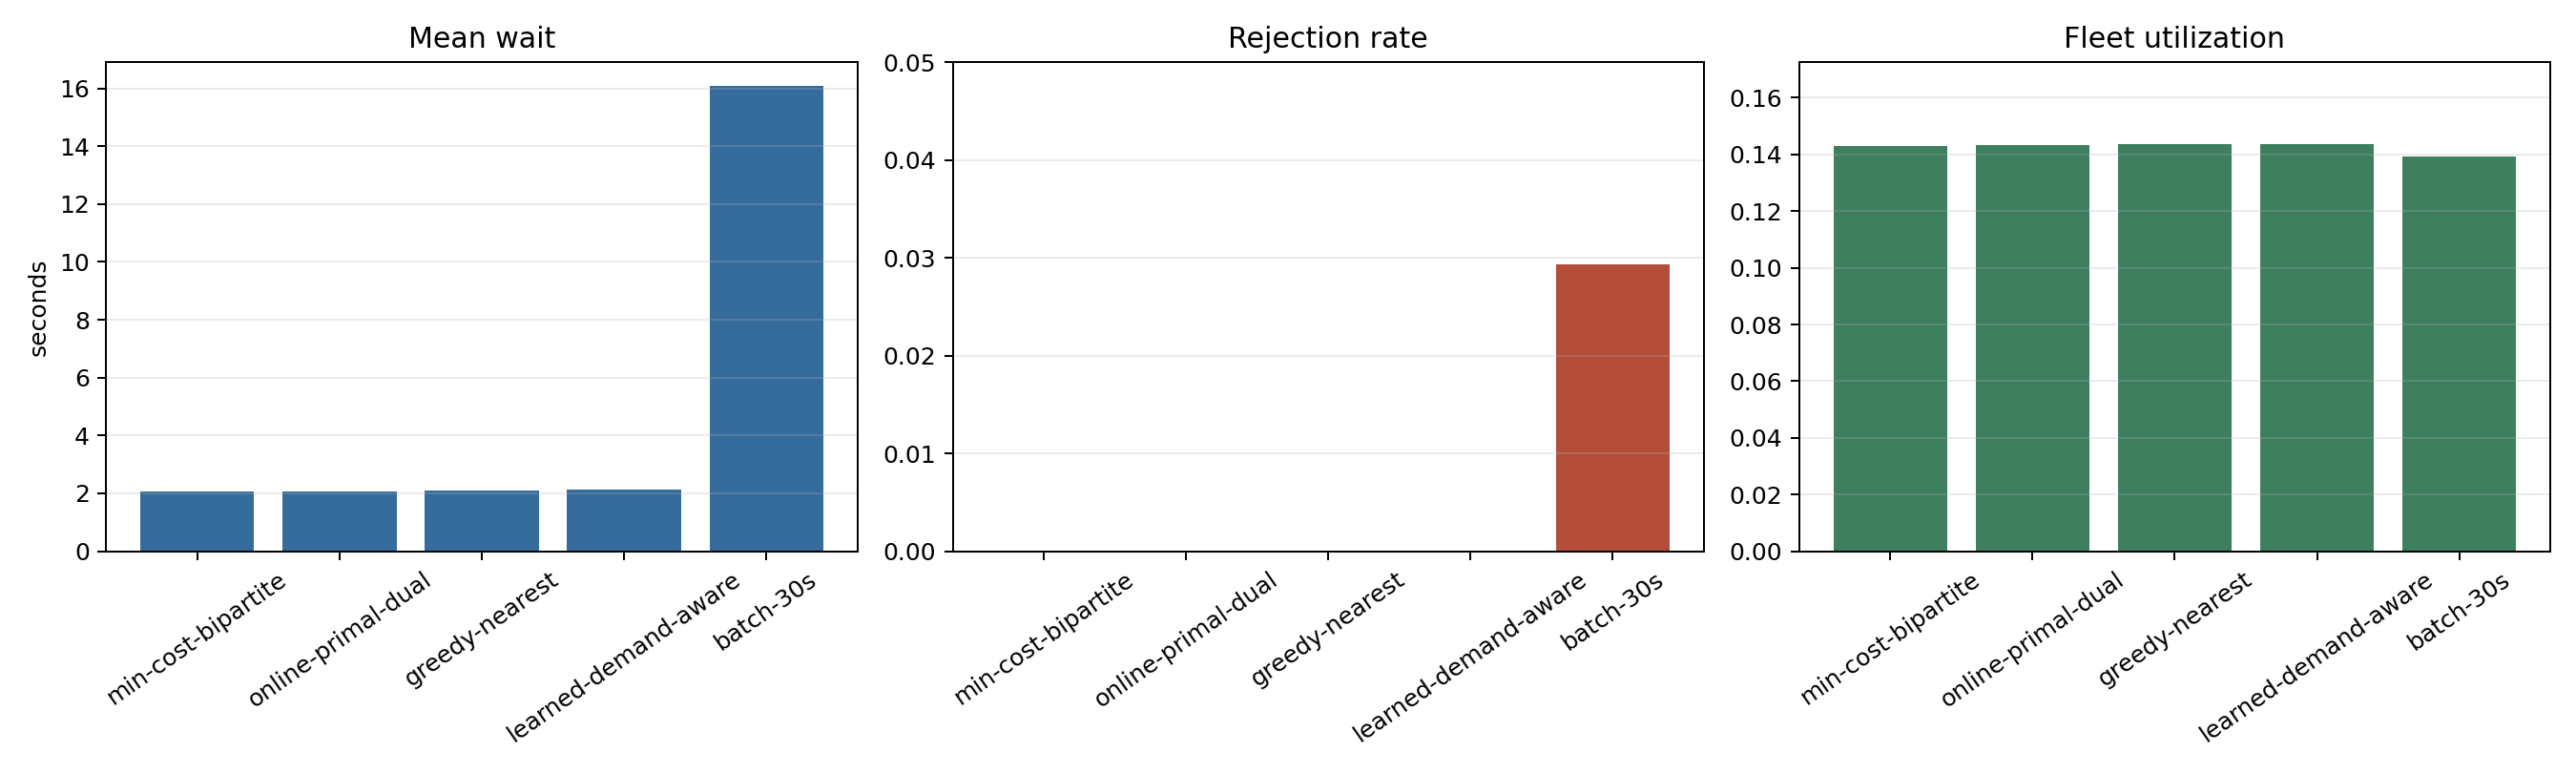
\includegraphics[width=\textwidth]{docs/figures/policy_summary.png}
}{
  \fbox{\parbox{0.85\textwidth}{\centering Run the experiment command and copy the figure to \texttt{docs/figures/policy\_summary.png}.}}
}
\caption{Comparison of mean wait time, rejection rate, and fleet utilization across dispatch policies.}
\label{fig:policy-summary}
\end{figure}

\section{Interpretation}

The min-cost bipartite policy generally provides the strongest immediate matching quality because it optimizes assignments jointly instead of greedily. Greedy matching is competitive when demand is light and the fleet is well distributed, but it lacks a mechanism for resolving conflicts among nearby riders. Batch matching exposes the central latency-quality tradeoff: delaying decisions can create better assignment opportunities, but it can also increase rider wait and rejection risk. The primal-dual and demand-aware policies are most interesting under spatial imbalance, where preserving supply in high-value zones can matter more than minimizing the current pickup distance alone.

\section{Limitations}

The simulator intentionally abstracts away several production details:

\begin{itemize}[nosep]
  \item travel times are graph distances rather than traffic-dependent estimates,
  \item drivers do not strategically reposition except for random idle movement,
  \item demand learning is an online heuristic rather than a trained model,
  \item cancellations, pooling, driver preferences, and pricing are not modeled,
  \item the grid graph is a simplified road network.
\end{itemize}

These abstractions keep the project focused on online matching and dispatch policy evaluation while leaving room for realistic extensions.

\section{Future Work}

Natural extensions include adversarial arrival sequences, competitive-ratio experiments, driver repositioning, fairness constraints across regions, larger road networks, sensitivity analysis over fleet size and batch interval, and learned demand models trained from historical traces.

\section{Conclusion}

The project demonstrates how online algorithms and matching theory can be translated into a practical simulator for real-time ride dispatch. It provides a clean experimental framework for comparing local greedy decisions, batch optimization, min-cost assignment, primal-dual-style pressure balancing, and demand-aware forecasting under stochastic arrivals.

\end{document}
